\section{Boundary Behavior of Hierarchical B-Splines}
\label{sec:32notAKnot}

As we have seen in the last section (see \cref{cor:hierSplittingBSpline}),
the hierarchical splitting equation \eqref{eq:hierSplittingUV}
only holds when restricting the function spaces to
$D_l^p = [h_l \tfrac{p-1}{2},\; 1 - h_l \tfrac{p-1}{2}]$,
which is for $p > 1$ a proper subset of the domain $[0, 1]$.
The implications of this fact on the approximation quality
of the hierarchical B-spline basis are severe.
In this section, we study the underlying reasons of the restriction and
we introduce a new B-spline basis that does not suffer from this issue.



\subsection{Approximation Power of Uniform Hierarchical B-Splines}
\label{sec:321approximation}

\paragraph{Interpolation of polynomials}

Splines are a piecewise generalization of polynomials.
Consequently, approximation spaces spanned by splines of degree $p$ should
at least contain all polynomials of degree $\le p$,
since the approximation power of splines should be at least as good
as that of polynomials.
Unfortunately, this statement is not true for the uniform B-splines
$\varphi_{l,i}^p$ as we have defined them in the last section.
A counterexample is given in \cref{fig:nakInterpolation},
in which a cubic polynomial $f$ is interpolated with
hierarchical cubic B-splines.
However, one can clearly deviations of the interpolant from the polynomial
near the boundary, where the relative error exceeds \SI{10}{\percent}.
The oscillations occur even in the interior of the
spline interpolation domain $D_l^p$.
Of course, this phenomenon does not improve the approximation quality
for other non-polynomial functions as well.

\begin{figure}
  \subcaptionbox{%
    Objective function \textcolor{C0}{$f$ \emph{(blue)}},
    interpolant \textcolor{C1}{$\tilde{f}$ \emph{(red, dashed)}},
    grid points \emph{(dots)}, and
    spline interpolation domain $D_3^p$ \emph{(thick line)}.%
  }[75mm]{%
    \includegraphics{nakInterpolation_1}%
  }%
  \hfill%
  \subcaptionbox{%
    Relative error $|(f - \tilde{f})/f|$ on a logarithmic scale.%
  }[75mm]{%
    \includegraphics{nakInterpolation_2}%
  }%
  \caption{%
    Hierarchical cubic B-splines $\varphi_{l',i'}^p$
    ($l' \le l$, $i' \in I_{l'}$, $p = 3$)
    fail to interpolate the cubic polynomial
    $f(x) := -10.2 x^3 + 14.7 x^2 - 5x + 0.7$
    on the grid of level $l = 3$.%
  }
  \label{fig:nakInterpolation}
\end{figure}

We can explain this as follows:
According to \thmref{cor:hierSplittingBSpline},
we have $S_l^p = \bigoplus_{l'=0}^l W_{l'}^p|_{D_l^p}$
with $p = 3$.
Since cubic polynomials as $f$ are cubic splines as well,
$f \in S_l^p$ and hence
$f \in \bigoplus_{l'=0}^l W_{l'}^p|_{D_l^p}$.
This means that there is a linear combination of hierarchical B-splines
$\varphi_{l',i'}^p$ ($l' \le l$, $i' \in I_{l'}$)
that interpolates $f$ exactly on the whole domain $D_l^p$
(not be confused with $\tilde{f}$ in \cref{fig:nakInterpolation},
which does not interpolate $f$ exactly in $D_l^p$).
However, in general, this interpolant is not equal $f$ outside
of $D_l^p$ (i.e., in $[0, 1] \setminus D_l^p$),
as \thmref{prop:splineSpace} only holds for $D_l^p$.
In particular, the interpolant evaluated at $x \in \{0, 1\}$ is not
equal to $f(x)$.
If we now force the additional interpolation conditions in
$x_{l,0} = 0$ and $x_{l,2^l} = 1$,
the resulting interpolant $\tilde{f}$ cannot be the same as the previous
interpolant,
which is why $f$ and $\tilde{f}$ differ inside $D_l^p$.

\paragraph{Schoenberg--Whitney conditions}

Formally, the unique existence of an interpolating spline is
described by the so-called Schoenberg--Whitney conditions:

\begin{proposition}[Schoenberg--Whitney conditions]
  Let $\ß\xi = (\xi_0, \dotsc, \xi_{m+p})$ be a knot sequence
  and $t_0, \dotsc, t_{m-1}$ a sequence of interpolation points with
  $\xi_p \le t_0 < \dotsb < t_{m-1} \le \xi_m$.
  Then, there exists a unique interpolating spline
  $s = \sum_{k=0}^{m-1} c_k b_{k,\ß\xi}^p$ for arbitrary data if and only if
  \begin{equation}
    \xi_k < t_k < \xi_{k+p+1},\quad
    k = 0, \dotsc, m - 1.
  \end{equation}
\end{proposition}

\begin{proof}
  See \cite{Hoellig13Approximation}.
\end{proof}

The Schoenberg--Whitney conditions require that the interpolation points
are contained in $D_l^p$.
In the example of $p = 3$ in \cref{fig:nakInterpolation},
the points $x = 0$ and $x = 1$ do not lie in~$D_l^p$.
For general degree $p$, the first $\tfrac{p-1}{2}$ and the
last $\tfrac{p-1}{2}$ grid points of level $l$ are missing from $D_l^p$,
thus violating the Schoenberg--Whitney conditions.
One possible remedy would be to move these interpolation points inside
$D_l^p$ without changing the corresponding basis functions
(i.e., the knots would stay the same) \cite{Hoellig13Approximation}.
For instance in the cubic case, we could move $x = 0$ and $x = 1$ to
$x = 1.5 h_l$ and $x = 1 - 1.5 h_l$, respectively.
However, with this approach, we would not be able to interpolate
boundary values.
In addition, the condition of the interpolation problem will most likely
worsen if we place interpolation points near the end of the supports
of the corresponding basis functions.

\paragraph{Restriction to spline subspaces}

As often, taking slightly a different view of the problem helps
to find a solution.
\newgsymbol{Slp01}{$S_l^{p,[0,1]}$}{%
  Spline space of degree $p$ on the grid
  $\{x_{l,i} \mid i = 0, \dotsc, 2^l\}$ of level $l$%
}%
Let $S_l^{p,[0,1]}$ denote the space of all splines of degree $p$
on the grid of level $l$, i.e., the space $S_\ß\xi^p$ with
\begin{equation}
  \label{eq:fullGridKnots}
  \xi_k := (k - p) h_l,\quad
  k = 0, \dotsc, m + p,\quad
  m := 2^l + p.
\end{equation}
We have $D_\ß\xi^p = [0, 1]$ for this choice of $\ß\xi$, i.e.,
the grid points $x_{l,i}$ ($i = 0, \dotsc, 2^l$) satisfy
the Schoenberg--Whitney conditions for the uniform B-spline basis.
Clearly, the sum $\bigoplus_{l'=0}^l W_l^p$ is a subspace of $S_l^{p,[0,1]}$,
but it cannot equal $S_l^{p,[0,1]}$ due to
\begin{equation}
  \dim \bigoplus_{l'=0}^l W_l^p
  = 2^l + 1
  < 2^l + p
  = m
  = \dim S_l^{p,[0,1]},\quad
  p > 1,
\end{equation}
by \thmref{prop:splineSpace}.
There are too few nodal (and hierarchical) basis functions to
span the whole spline space $S_l^{p,[0,1]}$.

The key idea is now to impose additional $(p - 1)$ boundary conditions
on the basis functions to restrict $S_l^{p,[0,1]}$ to a reasonable subspace
with the correct dimension $(2^l + p) - (p - 1) = 2^l + 1$.
``Reasonable'' means that besides this dimension constraint,
two requirements should be met:
First, the Schoenberg-Whitney conditions should be satisfied for
the new subspace and the grid of level $l$.
Second, the new subspace should contain all polynomials of degree $\le p$,
eliminating the issue discussed in \cref{fig:nakInterpolation}
in the process.



\subsection{Hierarchical Not-A-Knot B-Splines}
\label{sec:322NAKBSplines}

\paragraph{Not-a-knot conditions}

A suitable subspace can be obtained by incorporating the
so-called \term{not-a-knot boundary conditions} into $S_l^{p,[0,1]}$.
For the cubic case $p = 2$,
for which we need two conditions,
the not-a-knot conditions demand that
$\frac{\diff^3}{\dx^3} s$ is continuous at the first and last
interior knot $x_{l,1} = h_l$ and $x_{l,2^l-1} = 1 - h_l$
for all splines $s$ in the subspace.
Equivalently, $x_{l,1}$ and $x_{l,2^l-1}$ are effectively removed from the
knot sequence (hence ``not-a-knot''),
as this is equivalent to requiring that
$s$ is a cubic polynomial on $[0, x_{l,2}]$ and $[x_{l,2^l-2}, 1]$.
For general degree $p$ (in which we need $(p - 1)$ conditions),
we require that the $p$-th derivative $\frac{\diff^p}{\dx^p} s$
is continuous at the first $\tfrac{p-1}{2}$ and the last $\tfrac{p-1}{2}$
inner grid points
\begin{equation}
  \label{eq:removedNAKKnots}
  x_{l,i},\quad
  i \in \{1, \dotsc, \tfrac{p-1}{2}\} \cup
  \{2^l - \tfrac{p-1}{2}, \dotsc, 2^l - 1\},
\end{equation}
which is equivalent to removing these knots from the knot sequence $\ß\xi$,
or, alternatively, to requiring that $s$ is a polynomial
of degree $\le p$ on $[0, x_{l,(p+1)/2}]$ and on $[x_{l,2^l-(p+1)/2}, 1]$.

\newgsymbol{.nak}{$\cdot^\notaknot$}{%
  Superscript for ``Not-a-knot (knot sequence/basis
  function/function space/interpolant)''%
}%
\newgsymbol{xilpnak}{$\ß\xi_l^{p,\notaknot}$}{%
  Knot sequence
  for nodal not-a-knot B-splines of level $l$, degree $p$%
}%
\newgsymbol{Slpnak}{$S_l^{p,\notaknot}$}{%
  Spline space $:= S_{\ß\xi_l^{p,\notaknot}}^p$
  (spanned by the nodal not-a-knot B-splines of level $l$, degree $p$)%
}%
The knot sequence $\ß\xi_l^{p,\notaknot}$
with not-a-knot boundary conditions is defined as follows:
\begin{subequations}
  \begin{gather}
    \ß\xi_l^{p,\notaknot}
    := (\xi_{l,0}^{p,\notaknot}, \dotsc,
    \xi_{l,m+p}^{p,\notaknot}),\quad
    m := 2^l + 1,\\
    \xi_{l,k}^{p,\notaknot}
    :=
    \begin{cases}
      x_{l,k-p},&
      k = 0, \dotsc, p,\\
      x_{l,k-(p+1)/2},&
      k = p + 1, \dotsc, 2^l,\\
      x_{l,k-1},&
      k = 2^l + 1, \dotsc, 2^l + p + 1.
    \end{cases}
  \end{gather}
\end{subequations}
This knot sequence $\ß\xi_l^{p,\notaknot}$
can be obtained by removing the knots
given in \eqref{eq:removedNAKKnots} from the
knot sequence \eqref{eq:fullGridKnots} for the full grid of level $l$.
The resulting spline space
\begin{equation}
  S_l^{p,\notaknot}
  := S_{\ß\xi_l^{p,\notaknot}}^p
\end{equation}
is a subspace
of $S_l^{p,[0,1]}$ with the correct dimensionality:
\begin{equation}
  \dim \bigoplus_{l'=0}^l W_l^p
  = 2^l + 1
  = \dim S_l^{p,\notaknot}.
\end{equation}
The new space $S_l^{p,\notaknot}$ satisfies our two requirements:
First, the spline interpolation domain of $S_l^{p,\notaknot}$
equals the whole interval.
This means that the Schoenberg--Whitney conditions are satisfied
for $S_l^{p,\notaknot}$, since all interpolation points
(grid points) lie within $D_{\ß\xi_l^{p,\notaknot}}^p = [0, 1]$.
Second, $S_l^{p,\notaknot}$ still contains all polynomials of
degree $\le p$, as we have only removed knots compared to $S_l^{p,[0,1]}$.

\begin{figure}
  \includegraphics{splineSpace_3}%
  \caption{%
    Not-a-knot knot sequence $\ß\xi_l^{p,\notaknot}$
    \emph{(ticks on horizontal axis)}
    and corresponding nodal cubic not-a-knot B-splines ($p = 3$)
    of level $l = 3$.
    In the domain $[0, 1]$ \emph{(delimited by dashed lines)},
    the first $\tfrac{p-1}{2}$ and the last $\tfrac{p-1}{2}$ points
    of the set of grid points $\Omega_l$
    \emph{\textcolor{mittelblau}{(blue dots)}}
    have been removed from the set of knots.
    The spline interpolation domain $D_{\ß\xi_l^{p,\notaknot}}^p$
    \emph{(thick line)}
    equals the whole domain $[0, 1]$.%
  }%
  \label{fig:splineSpaceNotAKnot}%
\end{figure}

However, $\bigoplus_{l'=0}^l W_l^p$ is not a subspace of
$S_l^{p,\notaknot}$ anymore,
as the hierarchical basis functions $\varphi_{l',i'}^p$ are not
not-a-knot splines (due to the additional knots that we removed from
$S_l^{p,\notaknot}$).
For this reason,
we have to incorporate the not-a-knot boundary conditions into the
hierarchical basis.

Before defining the new hierarchical basis functions,
let us first make two additional observations.
First, $\ß\xi_l^{p,\notaknot}$ coincides with the
uniform knot sequence $\ß\xi_l^p$ of \thmref{cor:nodalBSplineSpace}
for the piecewise linear case of $p = 1$.
This is intuitively clear:
For this case,
we do not need to remove any knots as the hierarchical splitting already
holds for the full domain by \cref{cor:hierSplittingHat}.
Second, the removal of these knots is only possible if $p + 1 \le 2^l$,
which is equivalent to $l \ge \lceil\log_2(p+1)\rceil$.
For coarser levels,
there are not enough interior knots that could be removed.
Without any special treatment,
we would not be able to obtain enough basis functions to span the spline space.

\paragraph{Definition of hierarchical not-a-knot B-splines}

\newgsymbol{Lli}{$L_{l,i}$}{%
  Lagrange polynomial of level $l$, index $i$%
}%
For the definition of \term{hierarchical not-a-knot B-splines}
$\varphi_{l,i}^{p,\notaknot}$ based on \thmref{def:nonUniformBSpline},
we use global Lagrange polynomials for the coarser levels:
\begin{subequations}
  \begin{gather}
    \varphi_{l,i}^{p,\notaknot}
    :=
    \begin{cases}
      L_{l,i},&
      l < \lceil\log_2(p+1)\rceil,\\
      b_{i,\ß\xi_l^{p,\notaknot}}^p,&
      l \ge \lceil\log_2(p+1)\rceil,
    \end{cases}\quad
    l \in \NN_0,\quad
    i \in I_l,\\
    L_{l,i}\colon [0, 1] \to \RR,\quad
    L_{l,i}(x)
    := \prod_{\substack{i'=0,\dotsc,2^l\\i'\not=i}}
    \frac{x - x_{l,i'}}{x_{l,i} - x_{l,i'}}.
  \end{gather}
\end{subequations}
The hierarchical not-a-knot B-spline basis is shown for the
cubic case $p = 3$ in \cref{fig:notAKnotBSpline}.
The function $L_{l,i}$ is the $i$-th Lagrange polynomial of level $l$,
that is,
the unique polynomial of degree $\le 2^l$ that interpolates the data
$\{(x_{l,i'}, \delta_{i,i'}) \mid i' = 0, \dotsc, 2^l\}$.
\newgsymbol{deg}{$\deg f$}{%
  Degree of the polynomial $f$%
}%
Since its degree $\deg L_{l,i}$ is bounded by $2^l$,
we have $\deg L_{l,i} < p + 1$,
as the Lagrange polynomials are employed only when
$l < \lceil\log_2(p+1)\rceil$.
Due to $2^l$ even (when $l \ge 1$) and $p$ odd,
we can conclude from $\deg L_{l,i} \le 2^l \le p$ that actually
$\deg L_{l,i} \le 2^l < p$
(for $p > 1$; for $p = 1$, the case $l = 0$ is the exception).

\begin{figure}
  \subcaptionbox{%
    Nodal not-a-knot B-splines
    $\varphi_{l,i}^{p,\notaknot}$ ($i \in I_l$)
    and grid points $x_{l,i}$ \emph{(dots)}.%
  }[70mm]{%
    \includegraphics{hierarchicalBSpline_5}%
  }%
  \hfill%
  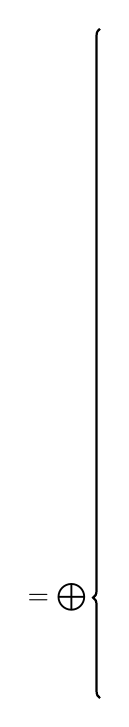
\begin{tikzpicture}
    \draw[decorate,thick,decoration={brace,aspect=0.15}] (0,-8.5) -- (0,0);
    \node[anchor=east,inner sep=0mm] at (-0.15,-7.225) {$= \bigoplus$};
  \end{tikzpicture}%
  \hfill%
  \subcaptionbox{%
    Hierarchical not-a-knot B-splines
    $\varphi_{l',i'}^{p,\notaknot}$ ($l' \le l$, $i' \in I_{l'}$)
    and grid points $x_{l',i'}$ \emph{(dots)}.%
  }[74mm]{%
    \includegraphics{hierarchicalBSpline_6}%
  }%
  \caption{%
    Univariate nodal and hierarchical cubic not-a-knot B-splines ($p = 3$)
    up to level $l = 3$.
    The nodal space $V_l^{p,\notaknot}$,
    which coincides with the not-a-knot spline space $S_l^{p,\notaknot}$,
    decomposes into the direct sum
    of the hierarchical subspaces $W_{l'}^{p,\notaknot}$ ($l' \le l$).
    The knots of each level $l'$ are given by removing the
    first $\tfrac{p-1}{2}$ and last $\tfrac{p-1}{2}$
    inner points \emph{(crosses)}
    from the set of grid points $x_{l',i'}$
    ($i' = 0, \dotsc, 2^{l'}$).%
  }%
  \label{fig:notAKnotBSpline}%
\end{figure}

The motivation for using Lagrange polynomials for coarse levels
is that they form a basis of the polynomial space
and that they can be implemented and calculated quickly.
However, the specific choice of basis functions for the levels
$l < \lceil\log_2(p + 1)\rceil$ is arbitrary,
as long as these functions are linearly independent
(of each other and of the ``true'' not-a-knot B-splines
$\varphi_{l,i}^{p,\notaknot}$, $l \ge \lceil\log_2(p+1)\rceil$)
and contained in the space $S_l^{p,\notaknot}$.

\paragraph{Implementation}

Note that in each level $l \ge \lceil\log_2(p+1)\rceil$,
only the first $\tfrac{p+1}{2}$
(indices $i = 1, 3, \dotsc, p$)
and the last $\tfrac{p+1}{2}$
(indices $i = 2^l - p, 2^l - p + 2, \dotsc, 2^l - 1$)
hierarchical basis functions $\varphi_{l,i}^{p,\notaknot}$
differ from $\varphi_{l,i}^p$,
i.e., we have
\begin{equation}
  \varphi_{l,i}^{p,\notaknot} = \varphi_{l,i}^p,\quad
  i = p + 2,\; p + 4,\; \dotsc,\; 2^l - p - 2.
\end{equation}
This means that we can reuse uniform B-spline code
for the inner functions.
Due to $\varphi_{l,i}^{p,\notaknot}(x) = \varphi_{l,2^l-i}^{p,\notaknot}(1-x)$
(because of the symmetry of $\ß\xi_l^{p,\notaknot}$),
we only have to implement $\tfrac{p+1}{2}$ not-a-knot B-splines per level $l$.
As $\varphi_{l,i}^{p,\notaknot}$ and $\varphi_{l+1,i}^{p,\notaknot}$
use the same knots up to an affine transformation for $l$ large enough
($l \ge 3$ suffices for $p = 3$),
we only have to implement a number of special case for coarse levels $l$.
In other words, the not-a-knot approach is ``minimally invasive''
with respect to an implementation that already uses uniform B-splines.

\paragraph{Hierarchical splitting}

The main benefit of the hierarchical not-a-knot B-spline basis
is the validity of the hierarchical splitting.
Again usual, we define $V_l^{p,\notaknot}$ and $W_l^{p,\notaknot}$
as the nodal and the hierarchical not-a-knot subspace of level $l$,
respectively.

\begin{proposition}[hierarchical splitting for not-a-knot B-splines]
  \label{prop:hierSplittingNAKBSplineUV}
  \newgsymbol{Pp}{$P^p$}{%
    Space of all polynomials of degree $\le p$ on $[0, 1]$%
  }%
  The hierarchical splitting \eqref{eq:hierSplittingUV}
  holds for the hierarchical not-a-knot B-spline basis:
  \begin{equation}
    S_l^{p,\notaknot}
    = V_l^{p,\notaknot}
    = \bigoplus_{l'=0}^l W_{l'}^{p,\notaknot},
  \end{equation}
  where for $l < \lceil\log_2(p+1)\rceil$, $S_l^{p,\notaknot}$
  is defined as the space $P^{2^l + 1}$ of polynomials of degree
  $\le 2^l + 1$ on $[0, 1]$
  (for $l \ge \lceil\log_2(p+1)\rceil$,
  $S_l^{p,\notaknot}$ is the not-a-knot spline space).
\end{proposition}

\begin{proof}
  For $l < \lceil\log_2(p+1)\rceil$, all
  three spaces coincide with $P^{2^l + 1}$ and nothing is to prove.
  
  For $l \ge \lceil\log_2(p+1)\rceil$,
  we check the two conditions of \thmref{lemma:hierSplittingUV}.
  First, the hierarchical subspace $W_{l'}^{p,\notaknot}$ ($l' \le l$)
  is a subspace of $S_l^{p,\notaknot} = V_l^{p,\notaknot}$.
  This is a conclusion of \thmref{prop:splineSpace}, as
  every function $\varphi_{l',i'}^{p,\notaknot}$ ($i' \in I_{l'}$)
  is continuous on $[0, 1]$, a polynomial on every knot interval of
  $\ß\xi_l^{p,\notaknot}$, and at the knots themselves
  at least $(p - 1)$ times continuously differentiable.
  
  Second, the hierarchical functions $\varphi_{l',i'}^{p,\notaknot}$
  ($l' \le l$, $i' \in I_{l'}$) are linearly independent.
  This can be shown similar to the proof of
  \thmref{prop:hierBSplineLinearlyIndependent}.
  The linear independence of the Lagrange polynomials
  can be checked by inserting grid points into a zero linear combination.
  The linear combination collapses and only one term remains,
  the coefficient corresponding to the grid point.
  Hence, all coefficients must vanish.
\end{proof}

\begin{corollary}
  \label{cor:hierSplittingNAKBSplineMV}
  It holds
  \begin{equation}
    S_\ßl^{\ßp,\notaknot}
    = V_\ßl^{\ßp,\notaknot}
    = \bigoplus_{\ßl'=\ß0}^\ßl W_{\ßl'}^{\ßp,\notaknot},
  \end{equation}
  where $S_\ßl^{\ßp,\notaknot}$ is the
  tensor product space of $S_{l_t}^{p_t,\notaknot}$
  ($t = 1, \dotsc, d$) as defined in \cref{prop:hierSplittingNAKBSplineUV}.
\end{corollary}

\begin{proof}
  Follows directly from \thmref{prop:splittingUVToMV}.
\end{proof}

\paragraph{Sparse grids with not-a-knot B-splines}

Regular sparse grid spaces using the new hierarchical not-a-knot basis
are defined analogously to the uniform case, i.e.,
\begin{equation}
  \label{eq:sparseGridRegularNAK}
  V_{n,d}^{\sparse,\ßp,\notaknot}
  := \bigoplus_{\norm{\ßl}_1 \le n} W_\ßl^{\ßp,\notaknot}.
\end{equation}
\newgsymbol{Pp!}{$P^\ßp$}{%
  Space of all $d$-variate polynomials of
  coordinate degree $\le \ßp$ on $[\ß0, \ß1]$%
}%
If the level $n$ is large enough, then $V_{n,d}^{\sparse,\ßp,\notaknot}$
contains the space $P^\ßp$ of all $d$-variate polynomials of
coordinate degree $\le \ßp$ on $[\ß0, \ß1]$
(i.e., functions $f\colon [0, 1] \to \RR$,
$f(\ßx) := \sum_{\ßq=\ß0}^\ßp c_\ßq \prod_{t=1}^d x_t^{q_t}$,
with $c_\ßq \in \RR$).
This means that in contrast to the uniform B-spline basis,
hierarchical not-a-knot B-splines on sparse grids are able to exactly
represent global polynomials on $[\ß0, \ß1]$.

\begin{corollary}
  If $n \ge \norm{\lceil\veclog_\ß2(\ßp + \ß1)\rceil}_1$,
  then $P^\ßp \subset V_{n,d}^{\sparse,\ßp,\notaknot}$.
\end{corollary}

\begin{proof}
  Let $\ßl := \lceil\veclog_\ß2(\ßp + \ß1)\rceil$ and $n \ge \norm{\ßl}_1$.
  By \cref{cor:hierSplittingNAKBSplineMV}, we have
  $\bigoplus_{\ßl' \le \ßl} W_\ßl^{\ßp,\notaknot} = S_\ßl^{\ßp,\notaknot}$.
  In addition, all $\ßl' \in \NN_0^d$ with $\ßl' \le \ßl$ satisfy
  $\norm{\ßl'}_1 \le n$ and thus,
  $\bigoplus_{\ßl' \le \ßl} W_\ßl^{\ßp,\notaknot} \subset
  V_{n,d}^{\sparse,\ßp,\notaknot}$ by \eqref{eq:sparseGridRegularNAK}.
  We conclude
  $P^\ßp \subset S_\ßl^{\ßp,\notaknot} \subset
  V_{n,d}^{\sparse,\ßp,\notaknot}$, which is the asserted claim.
\end{proof}



\subsection{Modified and Non-Uniform Hierarchical Not-A-Knot B-Splines}
\label{sec:323modifiedNAKBSplines}

\paragraph{Modified hierarchical not-a-knot B-splines}

Similar to uniform and Clenshaw--Curtis B-splines
(\cref{sec:31standardBSplines}),
it is possible to define a modified version of the
hierarchical not-a-knot B-spline basis to obtain
``reasonable'' boundary values without boundary points.
However, we cannot use \thmref{lemma:marsden} similarly to
\eqref{eq:modifiedBSplineConstruction}:
Due to the removal of knots, there is only a single
not-a-knot B-spline $\varphi_{l,0}^{p,\notaknot}$ left of
$\varphi_{l,1}^{p,\notaknot}$.
B-splines $\varphi_{l,i}^{p,\notaknot}$ with index $i < 0$
would be zero in $[0, 1]$.

While we are therefore not able to construct modified functions
whose second derivative vanishes in neighborhood of $x = 0$,
we can at least use $\varphi_{l,0}^{p,\notaknot}$ to let the
second derivative vanish in $x = 0$ itself:
\begin{equation}
  \label{eq:modifiedNotAKnotBSpline}
  \varphi_{l,i}^{p,\modified,\notaknot}(x)
  :=
  \begin{cases}
    1,&
    l = 1,\quad i = 1,\\
    \varphi_{l,1}^{p,\notaknot}(x)
    - \varphi_{l,0}^{p,\notaknot}(x)
    \dfrac{\frac{\diff^2}{\dx^2} \varphi_{l,1}^{p,\notaknot}(0)}%
    {\frac{\diff^2}{\dx^2} \varphi_{l,0}^{p,\notaknot}(0)},&
    l \ge 2,\quad i = 1,\\
    \varphi_{l,i}^{p,\notaknot}(x),&
    l \ge 2,\quad i \in I_l \setminus \{1, 2^l - 1\},\\
    \varphi_{l,1}^{p,\modified,\notaknot}(1 - x),&
    l \ge 2,\quad i = 2^l - 1.
  \end{cases}
  \hspace*{-2mm}
\end{equation}
The resulting modified hierarchical Clenshaw--Curtis not-a-knot B-spline basis
$\varphi_{l,i}^{p,\modified,\notaknot}$ is shown with dashed lines
in \cref{fig:modifiedNotAKnotBSpline}.
As before, we have to implement $\varphi_{l,1}^{p,\modified,\notaknot}$
only for a single level $l$, as modified functions of higher levels
are the same up to an affine parameter transformation.
Note again that for $p \ge 5$, we would have to modify additional
interior B-splines as the interior of their support then extends to the
boundary of $[0, 1]$.
We refrain from doing so to keep the definition
\eqref{eq:modifiedNotAKnotBSpline} simple.

\paragraph{Non-uniform hierarchical not-a-knot B-splines}

The not-a-knot construction is completely independent from the
distribution of the grid points at hand.
Consequently, we can define hierarchical not-a-knot B-splines
for non-uniform distributions.
For instance, to define not-a-knot B-splines for the
Chebyshev points in \cref{sec:314nonUniform},
we first specify the knot sequence as
\begin{subequations}
  \begin{gather}
    \ß\xi_l^{p,\clenshawcurtis,\notaknot}
    := (\xi_{l,0}^{p,\clenshawcurtis,\notaknot}, \dotsc,
    \xi_{l,m+p}^{p,\clenshawcurtis,\notaknot}),\quad
    m := 2^l + 1,\\
    \xi_{l,k}^{p,\clenshawcurtis,\notaknot}
    :=
    \begin{cases}
      x_{l,k-p}^\clenshawcurtis,&
      k = 0, \dotsc, p,\\
      x_{l,k-(p+1)/2}^\clenshawcurtis,&
      k = p + 1, \dotsc, 2^l,\\
      x_{l,k-1}^\clenshawcurtis,&
      k = 2^l + 1, \dotsc, 2^l + p + 1,
    \end{cases}
  \end{gather}
\end{subequations}
and then define hierarchical not-a-knot Clenshaw--Curtis B-splines as
\begin{subequations}
  \begin{gather}
    \varphi_{l,i}^{p,\clenshawcurtis,\notaknot}
    :=
    \begin{cases}
      L_{l,i}^\clenshawcurtis,&
      l < \lceil\log_2(p+1)\rceil,\\
      b_{i,\ß\xi_l^{p,\clenshawcurtis,\notaknot}}^p,&
      l \ge \lceil\log_2(p+1)\rceil,
    \end{cases}\quad
    l \in \NN_0,\quad
    i \in I_l,\\
    L_{l,i}^\clenshawcurtis\colon [0, 1] \to \RR,\quad
    L_{l,i}^\clenshawcurtis(x)
    := \prod_{\substack{i'=0,\dotsc,2^l\\i'\not=i}}
    \frac{x - x_{l,i'}^\clenshawcurtis}%
    {x_{l,i}^\clenshawcurtis - x_{l,i'}^\clenshawcurtis}.
  \end{gather}
\end{subequations}
This definition can even be combined with modification
of hierarchical not-a-knot B-splines as discussed above.
We can use exactly the same approach as in
\eqref{eq:modifiedNotAKnotBSpline}, if we replace the
not-a-knot basis functions with their non-uniform not-a-knot counterparts
(not-a-knot Clenshaw--Curtis B-splines in the above example).
The hierarchical not-a-knot Clenshaw--Curtis B-spline basis of
cubic degree and the corresponding modified functions are plotted in
\cref{fig:clenshawCurtisNotAKnotBSpline}.

\begin{figure}
  \subcaptionbox{%
    $\varphi_{l',i'}^{p,\notaknot}$,
    $\varphi_{l',i'}^{p,\modified,\notaknot}$
    \emph{(dashed)}, and $x_{l',i'}$ \emph{(dots)}.%
    \label{fig:modifiedNotAKnotBSpline}%
  }[73mm]{%
    \includegraphics{hierarchicalBSpline_7}%
  }%
  \hfill
  \subcaptionbox{%
    $\varphi_{l',i'}^{p,\clenshawcurtis,\notaknot}$,
    $\varphi_{l',i'}^{p,\modified,\clenshawcurtis,\notaknot}$
    \emph{(dashed)}, and $x_{l',i'}^\clenshawcurtis$ \emph{(dots)}.%
    \label{fig:clenshawCurtisNotAKnotBSpline}%
  }[76mm]{%
    \includegraphics{hierarchicalBSpline_8}%
  }%
  \caption{%
    Comparison of hierarchical uniform and Clenshaw--Curtis cubic not-a-knot
    B-splines $\varphi_{l',i'}^{p,\notaknot}$ and
    $\varphi_{l',i'}^{p,\clenshawcurtis,\notaknot}$
    ($l ' \le l$, $i' \in I_{l'}$, $p = 3$) up to level $l = 3$
    together with the respective modified versions
    $\varphi_{l',i'}^{p,\modified,\notaknot}$ and
    $\varphi_{l',i'}^{p,\modified,\clenshawcurtis,\notaknot}$
    \emph{(dashed)}.
    The knots of each level $l'$ are given by removing the
    first $\tfrac{p-1}{2}$ and last $\tfrac{p-1}{2}$
    inner points \emph{(crosses)}
    from the set of grid points $x_{l',i'}$ or
    $x_{l',i'}^\clenshawcurtis$
    ($i' = 0, \dotsc, 2^{l'}$), respectively.%
  }%
\end{figure}



\subsection{Other Approaches to Incorporate Boundary Conditions}
\label{sec:324naturalBoundary}

Not-a-knot boundary conditions are not the only approach
to obtain a subspace of $S_l^{p,[0,1]}$ with the right dimension $2^l - 1$.
Another possibility, which we want to discuss briefly, are
\term{natural boundary conditions}.
In the cubic case, for which they are usually formulated
\cite{Hoellig13Approximation},
these boundary conditions require that the
second derivatives $\frac{\diff^2}{\dx^2} \varphi_{l,i}$ of the
basis functions vanish at the boundary $x \in \{0, 1\}$.
To obtain the necessary number of $p - 1$ constraints also
for higher degrees $p$,
we require that all derivatives
$\frac{\diff^q}{\dx^q} \varphi_{l,i}$ of order
$q = 2, \dotsc, \tfrac{p+1}{2}$ vanish at $x \in \{0, 1\}$.

\newgsymbol{.nat}{$\cdot^\ntrl$}{%
  Superscript for ``Natural (basis
  function/function space/interpolant)''%
}%
Consequently, we can define hierarchical natural B-splines as
\begin{subequations}
  \begin{gather}
    \varphi_{l,i}^{p,\ntrl}(x)
    :=
    \begin{cases}
      L_{0,i}(x),&
      l = 0,\\
      \varphi_{l,i}^p +
      \sum_{j \in J_i^{p,\ntrl}} c_{l,i,j} \varphi_{l,j}^p,&
      l \ge 1,
    \end{cases}\quad
    l \in \NN_0,\quad
    i \in I_l,\\
    J_i^{p,\ntrl}
    := \{i+1-\tfrac{p+1}{2}, \dotsc, i-1\} \cup
    \{i+1, \dotsc, i-1+\tfrac{p+1}{2}\},
  \end{gather}
\end{subequations}
where the coefficients $c_{l,i,j} \in \RR$ are chosen such that
the natural boundary conditions are satisfied:
\begin{equation}
  \frac{\diff^q}{\dx^q} \varphi_{l,i}^{p,\ntrl}(x)
  = 0,\quad
  l \ge 1,\quad
  i \in I_l,\quad
  q = 2, \dotsc, \tfrac{p+1}{2},\quad
  x \in \{0, 1\}.
\end{equation}
\newgsymbol{suppo}{$\intsupp$}{%
  Interior of the support of a function (i.e., the non-zero set)%
}%
Note that the first half of the coefficients $c_{l,i,j} \in \RR$
($j < i$) vanish if the interior of the support of $\varphi_{l,i}^p$
does not contain $x = 0$
(i.e., $i > \tfrac{p+1}{2}$).
The second half of the coefficients~($j > i$) vanishes analogously
if $1 \notin \intsupp \varphi_{l,i}^p \iff i < 2^l - \tfrac{p+1}{2}$.
This means that as for the not-a-knot basis,
only the first $\tfrac{p+1}{2}$ and the last $\tfrac{p+1}{2}$
hierarchical functions have to be altered in each level.

\Cref{fig:naturalBSpline} shows the hierarchical natural spline basis.
The main disadvantage of natural boundary conditions is that
we are not able to replicate arbitrary polynomials exactly on $[0, 1]$
with this approach.
Only polynomials that satisfy natural boundary conditions themselves
(linear polynomials for example)
can be represented exactly with hierarchical natural B-splines.
For this reason, we do not further consider this basis in the
rest of the thesis.

\begin{SCfigure}
  \includegraphics{hierarchicalBSpline_9}%
  \caption{%
    Hierarchical cubic natural B-splines
    $\varphi_{l',i'}^{p,\ntrl}$
    ($l' \le l$, $i' \in I_{l'}$, $p = 3$) and
    grid points $x_{l',i'}$ \emph{(dots)} up to level $l = 3$.%
  }%
  \label{fig:naturalBSpline}%
\end{SCfigure}
